\chapter{Design}\label{C:des}

\section{Project Specifications and Justifications}
Given the results of the initial evaluation the project can now be constrained. It's main goals are to eliminate volume variation, control for droplet position, enable automation to reduced time between consecutive runs. It will not control, but provide data-logging for the environmental effectors; temperature, humidity, pressure.

From this there is a number of requirements to consider:

\begin{itemize}
    \item \textbf{Mechanical Stability}:
    \item \textbf{Droplet Position Repeatability}: 
    \item \textbf{Consistent and Variable Volume}: 
    \item \textbf{Process Automation}: 
    \item \textbf{System Expandability}:
\end{itemize}

The project will be evaluated on how it meets the above Specifications, its ability to control for volume and positional accuracy and repeatability as well as how it adds/improves automation, provides environmental data and allows extension.


\section{Drop Dispensing and Volume Control}

At the systems core is the liquid droplet dispensing hardware. The two core limitations of the initial setups manual syringe were fixed volume dispensing and the observed inconsistency in drop volume. In order to address these, alternative solution is required to provide a core that allows the rest of project to control and automate positioning, dispensing and liquid refilling. It was decided early on that the bulk of custom design would be focused on the motorisation hardware, custom mounting, and the driving software so the dispenser would be handled by a pre-existing product. The product selected for this is single channel electronic pipette from Labnet, P3600L-10. 

\begin{figure}[h]
    \centering
    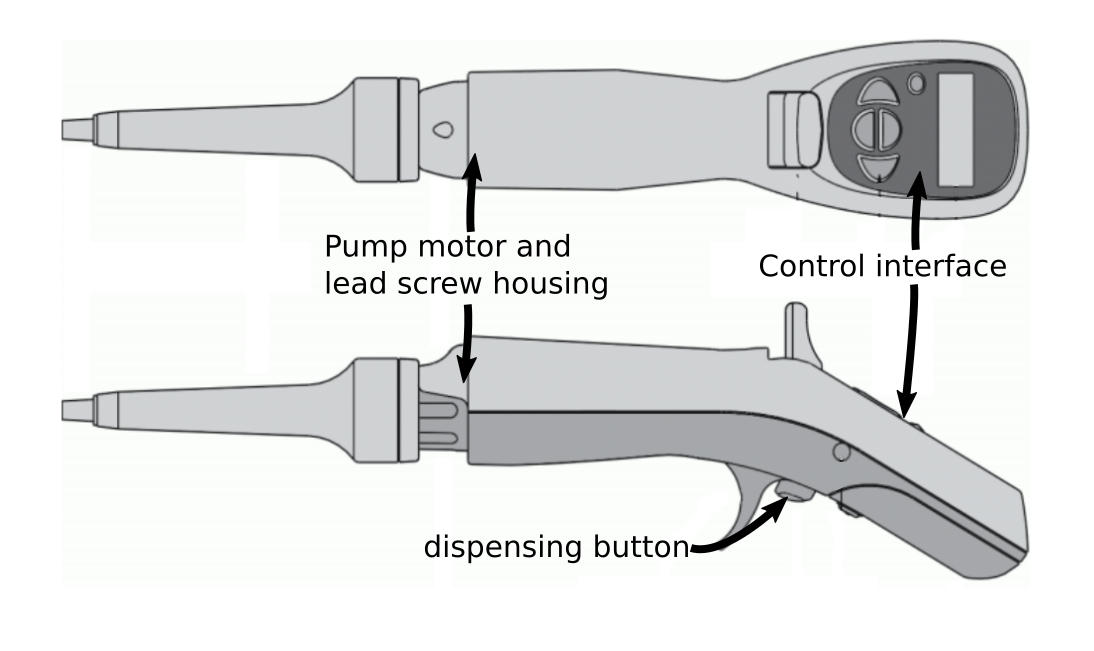
\includegraphics[width=0.4\textwidth]{img/epip.png}
    \caption{Labnet Excel P3600L-10}
    \label{fig:pip_dia}
\end{figure}

This product comes recalibrated and verified to dispense a droplet at a specified volume with at an accuracy of $\pm 4.0\rightarrow \pm 1.0 \%/\mu L$ over a the selection range of $0.5\mu L \; to \; 10\mu L$. This range represents the full range the pipette itself is capable of drawing and dispensing, configured via the front panel [see \ref{fig:pip_dia}], but an evaluation of the integrated system is required to confirm the mechanical stability is high enough prevent a high volume drop from prematurely detaching, as well as if its capable of depositing the minimum volume on the substrate.


Liquid refilling and dispensing is handled via the button on the back [\ref{fig:pip_dia}] and to enable the instrumentation to centrally control this, the planned approach was to break out the underlying switch contacts as GPIO inputs. The full process and results will be fully explored in this reports implementation system.


\section{Mechanical Design}

The goals for the mechanical aspects of this project are to provide a mounting interface to allow for the movement and positioning of the electronic pipette, mount to the optical XYZ stages, and transfer the driving force from the stepper motors to the instrumentations mechanisms.

All mechanisms share the requirements to fit compactly and correctly on the optical breadboard baseplate. Be designed in such a way to minimise backlash and prevent vibrations from propergating and resonating through the system. As this could interfere with droplet dispensing; increasing pipette tip overshoot and settling times, causes prematurely drop detachment and generally decreasing the key performance metrics.

\subsection{Rotating Pipette Mount}

The first half of the main assembly is Pipette Stage. In order to manoeuvre the pipette from reservoir to substrate stack, the pipette needs to be held at specific height and angle to roughly match the central stage (as it is Z adjustable) and rotate between these two points.

To achieve the mounting stage consists of three main parts: 
\begin{itemize}
    \item Pipette clamping and Angled mount: Responsible with securely fastening the e-pipette at the correct angle.
    \item Laser Cut Mounting Tower: Sets pipette height and connects pipette to motor.
    \item Motor shaft interface and Stage Fastening: Rotation is directly driven via the motor, thus the assembly is mounted to the motor shaft. 
\end{itemize}

Dimensional Specifications: Pipette height of 130mm (from breadboard) and angle of 36.25 degrees.
These specification are used to derive the full dimensions of the following assemblies.

The electronic pipette formfactor is ergonomic-hand to fit in human hand-so the clamping mechanism to fit it to the tower plate itself was challenging to design to successfully restrict its rotation and backlash. 3D printed PLA c-clamps were the perused approach to capitalise on the materials ability to deform and to aid in rapid implementation and testing.

\begin{figure}[h]
    \centering
    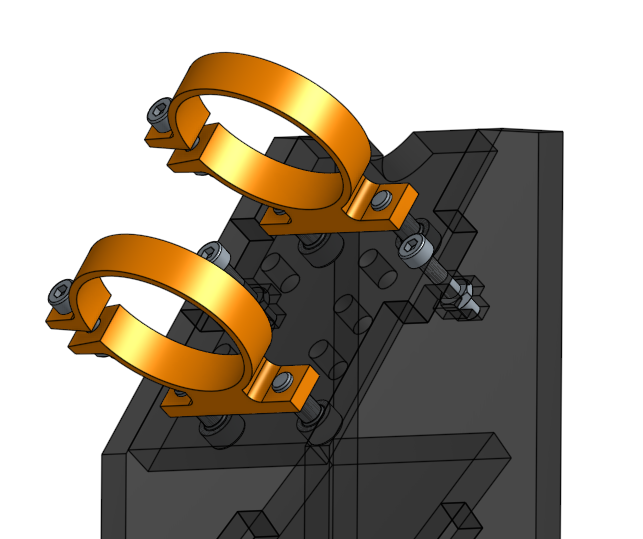
\includegraphics[width=0.4\textwidth]{img/pip_clamp.png}
    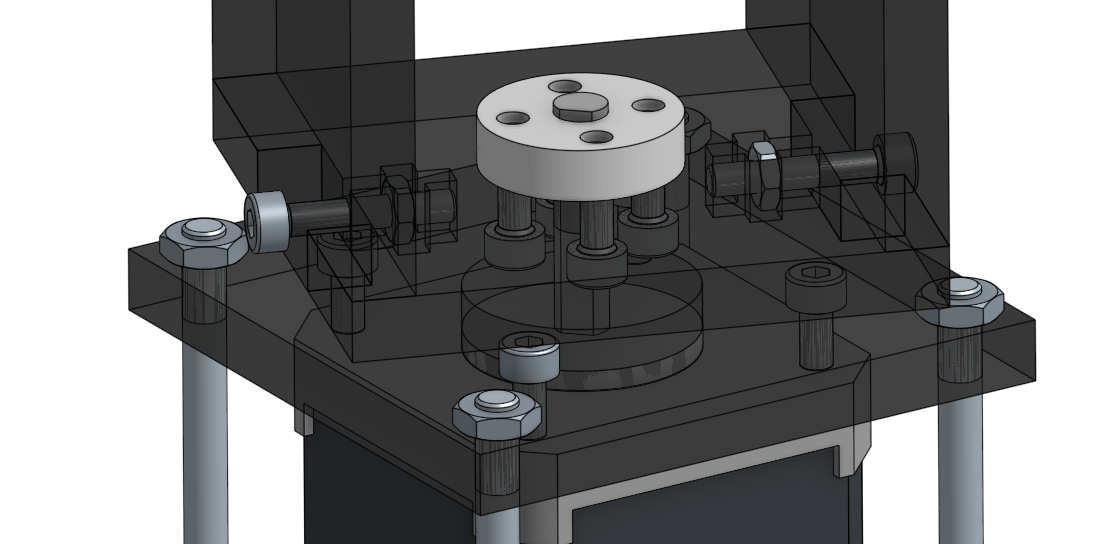
\includegraphics[width=0.4\textwidth]{img/tower_mount.png}
    \caption{Left: Pipette Clamps and Tower, Right: Towers base mounting to motor shaft}
    \label{fig:tower}
\end{figure}

The base design used to accomplish this was a 3D-printed ring clamp [Left:\ref{fig:tower}] meant to be tightened and fit to the unique form of the pipette body. A variety of ring sizes and gap distance were printed and test fitted. From this it was determined that a ring diameter of 32mm and a gap of 6mm fits and deforms to the shape of the pipette. However, there was still some rotation and slip so a notch was cut into the acrylic angle plate [Left:\ref{fig:tower}] to slot the pipettes support rest and a second ring clamp (36mm) attached lower down of the body.

 //TODO More detail on motor mounting?

\subsection{Z micrometer Control}

In order to control the the height of the pipette tip; to enable automated refilling and to place the dispensed droplet on to the substrate the Z height of the optical stage needs to be motorised. The Z height has a manual control in the form of an adjustment micrometer that allows for 10mm of travel, but this present the first problem in design.
The micrometer travels linearly throughout the adjustment, i.e. if the stage raises 10mm the knob will retract 10mm also. Due to this a custom shaft coupler is required to interface a fixed motor to the moving knob.

\begin{figure}[h]
    \centering
    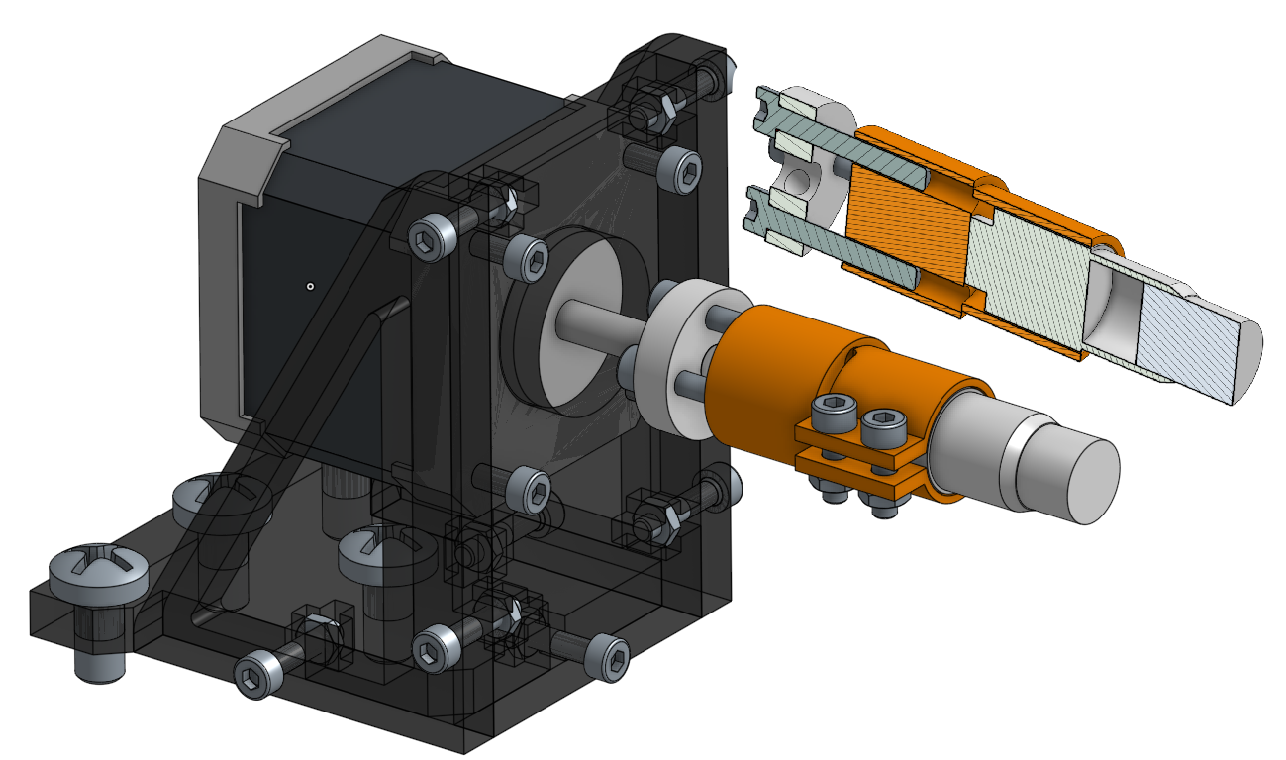
\includegraphics[width=0.4\textwidth]{img/z_control.png}
    \caption{Z Driving Motor and Sliding Shaft Coupler}
    \label{fig:z_coup}
\end{figure}

The figure above[\ref{fig:z_coup}] shows the assembled design. One end of the coupler is an extended c-clamp that mates with the knurls knobs of the micrometer and the other is a solid piece with 4 M3 clearance holes. These holes interface with a universal shaft-hub mount with 4 M3 machine screws that transfer the motors rotation and allow the coupler and knob to slide away over the course of a movement.

The key limitation of this design is that is constrains the XY position of the stage to a single setting. This is due to the motor being fastened to the breadboard baseplate more stability, alignment and vibration reduction. Because of this it moves the fine positioning to the other stages in the setup; substrate stack and cameras. 

\section{Electronic Design}

\subsection{Motors}
The motion required for the motors in this system is to provide rotation about the vertical axis to the mounted pipette, to swing from above the substrate to out of the camera view and over a refill reservoir, as well as continuous rotation to interface the Z axis control for droplet depositing and possible refilling.

Stepper motors allow for both precise position control without the need for a feedback system and are capable of continuous rotation. In comparison, brushed/brushless DC motors require encoders for positional control and servos may do either but not both continuous rotation and positioning.

NEMA17 standard sized steppers were chosen to best fit the dimensions of the XYZ optical stage (60mm plate to 40mm motor frame) with room for fastening hardware. That left two choices for the top R stage motor; full size 38mm high frame or shorter pancake frame. Even through the pancake frame would reduce the overall height of the system, the shaft length available for this motor is less only 7mm and would greatly restrict the mounting options of the tower to the motor. For this reason 2 NEMA17x38mm Stepper motors were chosen.

\subsection{Motor Driving}

\subsubsection*{The Requirements}
To drive the selected stepper motors, discrete step/direction style micro stepping drivers were chosen. This allows for the design to be flexible with its electronics placed to accommodate the experimental needs. Allows for a fairly agnostic choice for controller to supply the control signals, and standardised pinouts allow for requirement flexibility and replacements.

\begin{table}[h]
    \centering
    \begin{tabular}{|l|l|l|l|l|}
        \hline
        \textbf{}     & \textbf{A4988} & \textbf{DRV8825} & \textbf{STPIN820} & \textbf{DRV8834} \\ \hline
        Step Res      & 1/16           & 1/32             & 1/256             & 1/32             \\ \hline
        Logic Level   & 3V3/5V         & 3V3/5V           & 3V3/5V            & 3V3/5V           \\ \hline
        Current Limit & 1A             & 1.5A             & 0.9A              & 1.5A             \\ \hline
        Drive Voltage & 8-35V          & 8.2-45V          & 7-48V             & 2.5-10.8         \\ \hline
    \end{tabular}
    \caption{Comparison of considered drivers}
\end{table}

Main consideration for device choice are: micro step resolution, driving current limit (passively cooled), and configuration pinout.

\subsubsection*{The Choice}
The DRV8825 was ultimately chosen.
\begin{itemize}
    \item High microstepping resolution, lower than the STPIN820 but cheap high resolution driver are prone to step skipping \cite{step_book}
    \item Highest driving current as torque requirements are unknown for this design the headroom is nice even if it isn't use, especially as it will run cooler at lower power draw.
    \item It ranked above the DRV8834 due to it configuration pins (to set microstepping mode) as it provide all 3 pins without the requirement to leave pins floating as a setting thus allowing for full software control.
\end{itemize}

\newpage
\subsection{Environmental Monitoring}

Although the aim of this project is to only control the position and volume of the droplet in the experiment, to at least fully address the list of affector [covered in \ref{C:init_eval}] the environmental factors recorded are: \textbf{Temperature, Barometric Pressure, Relative Humidity}.

As this section of the project doesn't note share resources with the main motorised assembly it key design considerations were simplicity and function.
Therefore, the environmental monitor is not required to have any integration with the main controller or data logging capabilities.

To meets these requirements the monitor was decided to be a low power microcontroller + OLED display stack that polled environmental sensor peripherals. This would be battery powered and utilised low power sleep modes to extend lifetimes

To facilitate ease

\section{System Overview}

\begin{figure}[h]
    \centering
    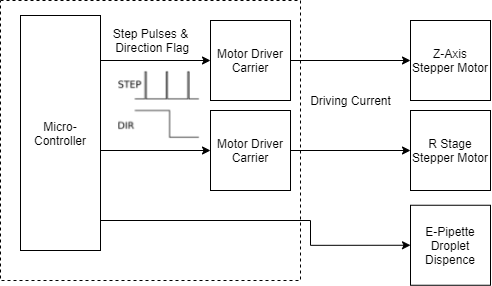
\includegraphics[width=0.4\textwidth]{img/ED_block_diag.png}
    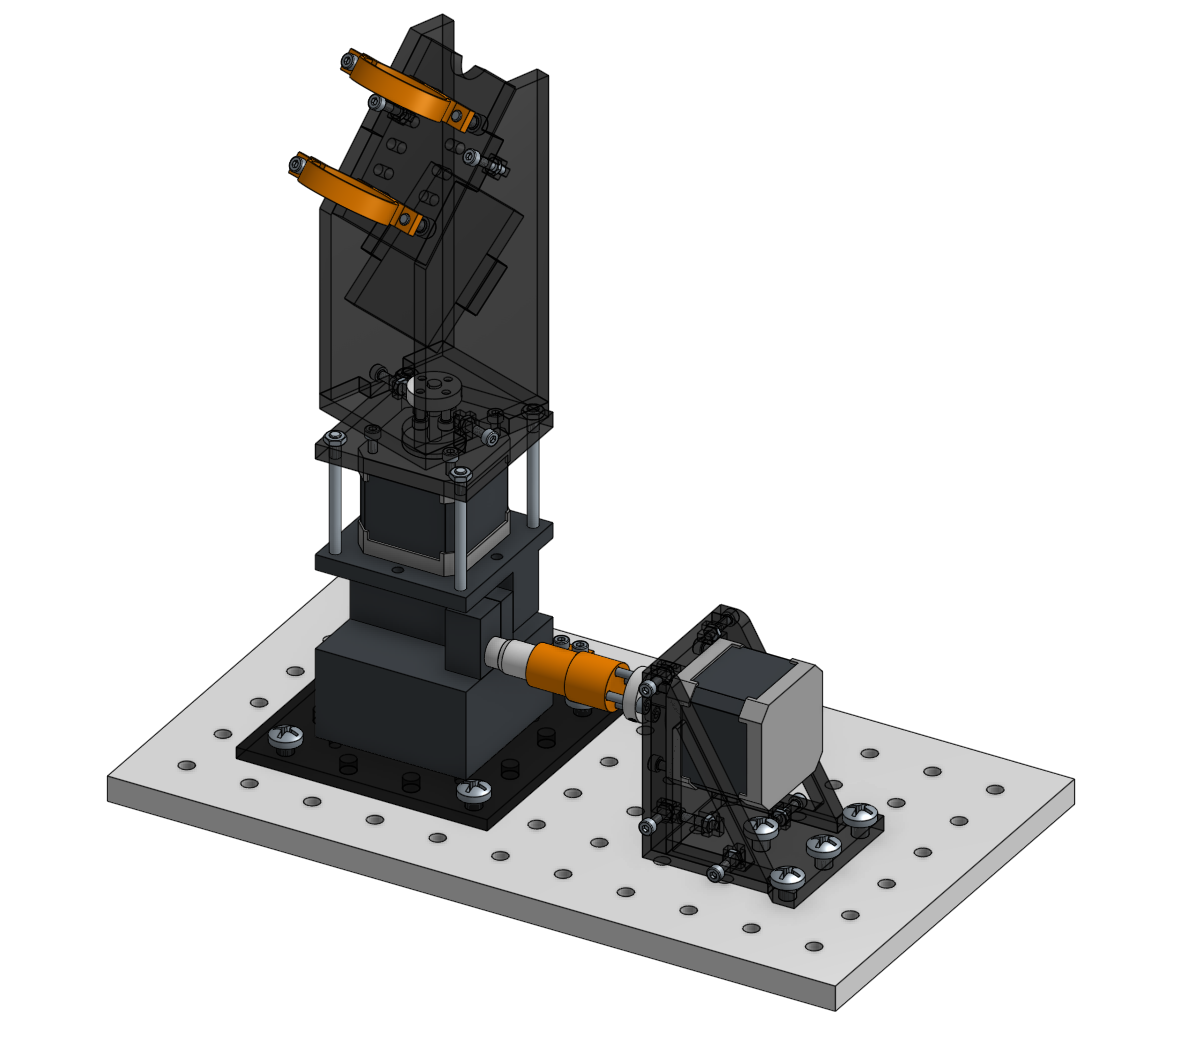
\includegraphics[width=0.4\textwidth]{img/full_mech.png}
\end{figure}